% Lines that start with a % are comments and are not included when the LaTeX file is converted to a pdf

% Set up the document class - this can be changed if a different format is required 
\documentclass[12pt,a4paper]{article}

% Include packages that contain additional features, for example including special mathematical characters and images in your document
\usepackage{amssymb,amsmath,graphicx}


\usepackage{geometry}
 \geometry{
 a4paper,
 total={170mm,257mm},
 left=20mm,
 top=20mm,
 }



% The beginning of the document...
\begin{document}

% Please change the following accordingly...
\centerline{\large Exercise sheet 3}\vspace{0.5em}
\centerline{\large by Maximilian Richter and Christian Heppe}\vspace{1em}

% Split the different exercises into different sections...
\section*{2. Neutrons in the gravitational field}

% To include a plot it must be in the same directory as the .tex file.
\subsection*{1. Asymptotic behaviour}
To observe the asymptotic behaviour of the Numerov-method, we plotted two solutions for $\epsilon=1$ and $\epsilon=2$ from $x=0$ to $x=30$ with a stepsize of $h=0.001$. As one can clearly see, the values go to positive or negative infinity, depending on the value of $\epsilon$.\\ 
% Remove the "%" in the following line and change the "plot.png" to the name of the plot to include.
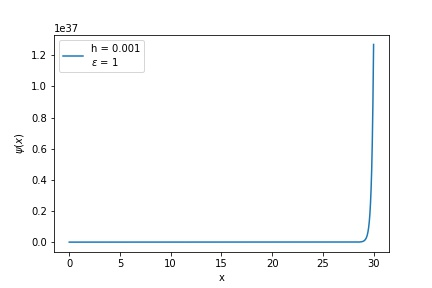
\includegraphics[width=8cm]{partb1.jpg}
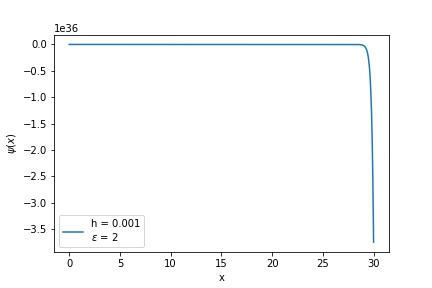
\includegraphics[width=8cm]{partb2.jpg}
\newline
\subsection*{2. Eigenvalues $\epsilon_n$ of Schrödinger's equation}
In order to determine the eigenvalues $\epsilon_n$ of Schrödinger's equation we used the property, that they belong to normalizable eigenfuctions with $\psi(x)\rightarrow0$ for $x\rightarrow\infty$. As one can see in part 1 of this exercise, the asymptote changes its sign from $\epsilon=1$ to $2$, this means there is an eigenvalue in between those values. With this approach we could determine the first four eigenvalues $\epsilon_n$ to 3 decimals after the comma. The values all have been found with a stepsize of $h=0.001$ for the algorithm.
\begin{align*}
\epsilon_1 &= 1.018\\
\epsilon_2 &= 3.248\\
\epsilon_3 &= 4.820\\
\epsilon_4 &= 6.163
\end{align*}
\subsection*{Extra: Solution for classical zone}
\begin{center}
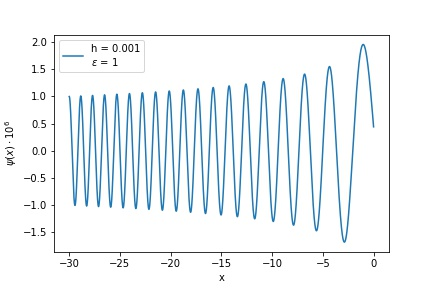
\includegraphics[width=8cm]{partb3.jpg}
\end{center}
\end{document}

